% Options for packages loaded elsewhere
\PassOptionsToPackage{unicode}{hyperref}
\PassOptionsToPackage{hyphens}{url}
%
\documentclass[
]{article}
\usepackage{lmodern}
\usepackage{amsmath}
\usepackage{ifxetex,ifluatex}
\ifnum 0\ifxetex 1\fi\ifluatex 1\fi=0 % if pdftex
  \usepackage[T1]{fontenc}
  \usepackage[utf8]{inputenc}
  \usepackage{textcomp} % provide euro and other symbols
  \usepackage{amssymb}
\else % if luatex or xetex
  \usepackage{unicode-math}
  \defaultfontfeatures{Scale=MatchLowercase}
  \defaultfontfeatures[\rmfamily]{Ligatures=TeX,Scale=1}
\fi
% Use upquote if available, for straight quotes in verbatim environments
\IfFileExists{upquote.sty}{\usepackage{upquote}}{}
\IfFileExists{microtype.sty}{% use microtype if available
  \usepackage[]{microtype}
  \UseMicrotypeSet[protrusion]{basicmath} % disable protrusion for tt fonts
}{}
\makeatletter
\@ifundefined{KOMAClassName}{% if non-KOMA class
  \IfFileExists{parskip.sty}{%
    \usepackage{parskip}
  }{% else
    \setlength{\parindent}{0pt}
    \setlength{\parskip}{6pt plus 2pt minus 1pt}}
}{% if KOMA class
  \KOMAoptions{parskip=half}}
\makeatother
\usepackage{xcolor}
\IfFileExists{xurl.sty}{\usepackage{xurl}}{} % add URL line breaks if available
\IfFileExists{bookmark.sty}{\usepackage{bookmark}}{\usepackage{hyperref}}
\hypersetup{
  pdftitle={EDDA - Assignment 1},
  hidelinks,
  pdfcreator={LaTeX via pandoc}}
\urlstyle{same} % disable monospaced font for URLs
\usepackage[margin=1in]{geometry}
\usepackage{color}
\usepackage{fancyvrb}
\newcommand{\VerbBar}{|}
\newcommand{\VERB}{\Verb[commandchars=\\\{\}]}
\DefineVerbatimEnvironment{Highlighting}{Verbatim}{commandchars=\\\{\}}
% Add ',fontsize=\small' for more characters per line
\usepackage{framed}
\definecolor{shadecolor}{RGB}{248,248,248}
\newenvironment{Shaded}{\begin{snugshade}}{\end{snugshade}}
\newcommand{\AlertTok}[1]{\textcolor[rgb]{0.94,0.16,0.16}{#1}}
\newcommand{\AnnotationTok}[1]{\textcolor[rgb]{0.56,0.35,0.01}{\textbf{\textit{#1}}}}
\newcommand{\AttributeTok}[1]{\textcolor[rgb]{0.77,0.63,0.00}{#1}}
\newcommand{\BaseNTok}[1]{\textcolor[rgb]{0.00,0.00,0.81}{#1}}
\newcommand{\BuiltInTok}[1]{#1}
\newcommand{\CharTok}[1]{\textcolor[rgb]{0.31,0.60,0.02}{#1}}
\newcommand{\CommentTok}[1]{\textcolor[rgb]{0.56,0.35,0.01}{\textit{#1}}}
\newcommand{\CommentVarTok}[1]{\textcolor[rgb]{0.56,0.35,0.01}{\textbf{\textit{#1}}}}
\newcommand{\ConstantTok}[1]{\textcolor[rgb]{0.00,0.00,0.00}{#1}}
\newcommand{\ControlFlowTok}[1]{\textcolor[rgb]{0.13,0.29,0.53}{\textbf{#1}}}
\newcommand{\DataTypeTok}[1]{\textcolor[rgb]{0.13,0.29,0.53}{#1}}
\newcommand{\DecValTok}[1]{\textcolor[rgb]{0.00,0.00,0.81}{#1}}
\newcommand{\DocumentationTok}[1]{\textcolor[rgb]{0.56,0.35,0.01}{\textbf{\textit{#1}}}}
\newcommand{\ErrorTok}[1]{\textcolor[rgb]{0.64,0.00,0.00}{\textbf{#1}}}
\newcommand{\ExtensionTok}[1]{#1}
\newcommand{\FloatTok}[1]{\textcolor[rgb]{0.00,0.00,0.81}{#1}}
\newcommand{\FunctionTok}[1]{\textcolor[rgb]{0.00,0.00,0.00}{#1}}
\newcommand{\ImportTok}[1]{#1}
\newcommand{\InformationTok}[1]{\textcolor[rgb]{0.56,0.35,0.01}{\textbf{\textit{#1}}}}
\newcommand{\KeywordTok}[1]{\textcolor[rgb]{0.13,0.29,0.53}{\textbf{#1}}}
\newcommand{\NormalTok}[1]{#1}
\newcommand{\OperatorTok}[1]{\textcolor[rgb]{0.81,0.36,0.00}{\textbf{#1}}}
\newcommand{\OtherTok}[1]{\textcolor[rgb]{0.56,0.35,0.01}{#1}}
\newcommand{\PreprocessorTok}[1]{\textcolor[rgb]{0.56,0.35,0.01}{\textit{#1}}}
\newcommand{\RegionMarkerTok}[1]{#1}
\newcommand{\SpecialCharTok}[1]{\textcolor[rgb]{0.00,0.00,0.00}{#1}}
\newcommand{\SpecialStringTok}[1]{\textcolor[rgb]{0.31,0.60,0.02}{#1}}
\newcommand{\StringTok}[1]{\textcolor[rgb]{0.31,0.60,0.02}{#1}}
\newcommand{\VariableTok}[1]{\textcolor[rgb]{0.00,0.00,0.00}{#1}}
\newcommand{\VerbatimStringTok}[1]{\textcolor[rgb]{0.31,0.60,0.02}{#1}}
\newcommand{\WarningTok}[1]{\textcolor[rgb]{0.56,0.35,0.01}{\textbf{\textit{#1}}}}
\usepackage{graphicx}
\makeatletter
\def\maxwidth{\ifdim\Gin@nat@width>\linewidth\linewidth\else\Gin@nat@width\fi}
\def\maxheight{\ifdim\Gin@nat@height>\textheight\textheight\else\Gin@nat@height\fi}
\makeatother
% Scale images if necessary, so that they will not overflow the page
% margins by default, and it is still possible to overwrite the defaults
% using explicit options in \includegraphics[width, height, ...]{}
\setkeys{Gin}{width=\maxwidth,height=\maxheight,keepaspectratio}
% Set default figure placement to htbp
\makeatletter
\def\fps@figure{htbp}
\makeatother
\setlength{\emergencystretch}{3em} % prevent overfull lines
\providecommand{\tightlist}{%
  \setlength{\itemsep}{0pt}\setlength{\parskip}{0pt}}
\setcounter{secnumdepth}{-\maxdimen} % remove section numbering
\ifluatex
  \usepackage{selnolig}  % disable illegal ligatures
\fi

\title{EDDA - Assignment 1}
\author{}
\date{\vspace{-2.5em}}

\begin{document}
\maketitle

\hypertarget{exercise-1}{%
\section{Exercise 1}\label{exercise-1}}

The data set birthweight.txt contains the birthweights of 188 newborn
babies. We are interested in finding the underlying (population) mean μ
of birthweights.

\textbf{a)} Check normality of the data. Compute a point estimate for μ.
Derive, assuming normality (irrespective of your conclusion about
normality od the data), a bounded 90\% confidence interval for μ.

To check normality for the data we use a qqplot, historgram, box plot
and shapiro-wilks test.

\begin{Shaded}
\begin{Highlighting}[]
\FunctionTok{par}\NormalTok{(}\AttributeTok{mfrow=}\FunctionTok{c}\NormalTok{(}\DecValTok{1}\NormalTok{,}\DecValTok{3}\NormalTok{))}
\NormalTok{data}\OtherTok{=}\FunctionTok{read.table}\NormalTok{(}\AttributeTok{file=}\StringTok{"data/birthweight.txt"}\NormalTok{,}\AttributeTok{header=}\ConstantTok{TRUE}\NormalTok{)}

\NormalTok{bw }\OtherTok{=}\NormalTok{ data}\SpecialCharTok{$}\NormalTok{birthweight}
\FunctionTok{hist}\NormalTok{(bw)}
\FunctionTok{qqnorm}\NormalTok{(bw)}
\FunctionTok{boxplot}\NormalTok{(bw)}
\end{Highlighting}
\end{Shaded}

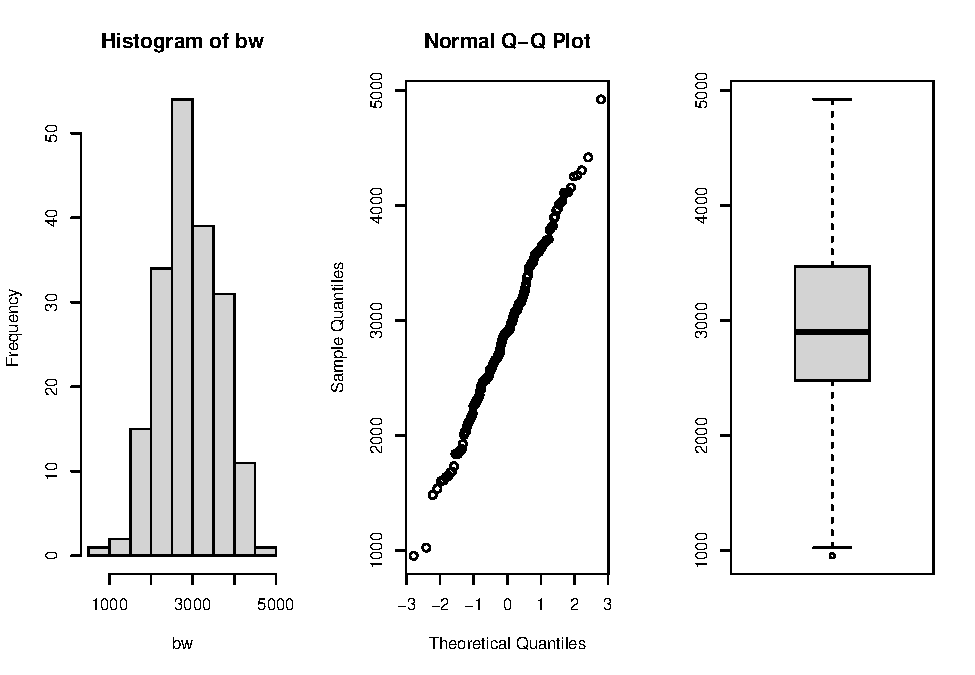
\includegraphics{Assignment-1_files/figure-latex/unnamed-chunk-1-1.pdf}

\begin{Shaded}
\begin{Highlighting}[]
\FunctionTok{shapiro.test}\NormalTok{(bw)}
\end{Highlighting}
\end{Shaded}

\begin{verbatim}
## 
##  Shapiro-Wilk normality test
## 
## data:  bw
## W = 0.99595, p-value = 0.8995
\end{verbatim}

The graphical methods show that the data is normal. The Shapiro-Wilk
test reinforces this assumption as it shows a p-value of 0.8995, meaning
that the H0 is not rejected and therefore the data is normal.
Furthermore, a point estimate for mu is conducted along side a 90\%
confidence interval.

\begin{Shaded}
\begin{Highlighting}[]
\NormalTok{m }\OtherTok{=} \FunctionTok{mean}\NormalTok{(bw)}
\NormalTok{sd }\OtherTok{=} \FunctionTok{sd}\NormalTok{(bw)}
\NormalTok{n }\OtherTok{=} \FunctionTok{length}\NormalTok{(bw)}
\NormalTok{error }\OtherTok{=} \FunctionTok{qnorm}\NormalTok{(}\FloatTok{0.95}\NormalTok{)}\SpecialCharTok{*}\NormalTok{sd}\SpecialCharTok{/}\FunctionTok{sqrt}\NormalTok{(n)}
\NormalTok{ci }\OtherTok{=} \FunctionTok{c}\NormalTok{(m}\SpecialCharTok{{-}}\NormalTok{error, m}\SpecialCharTok{+}\NormalTok{error)}
\NormalTok{m}
\end{Highlighting}
\end{Shaded}

\begin{verbatim}
## [1] 2913.293
\end{verbatim}

\begin{Shaded}
\begin{Highlighting}[]
\NormalTok{ci}
\end{Highlighting}
\end{Shaded}

\begin{verbatim}
## [1] 2829.618 2996.967
\end{verbatim}

\textbf{b)} An expert claims that the mean birthweight is bigger than
2800, verify this claim by using at-test.What is the outcome of the test
if you take α = 0.1? And other values of α?

A t-test is performed to verify the claim that the mean birthweight is
bigger than 2800. The t-test shows a p-value of 0.014. This means that
this claim is significant for an α of 0.1. The claim is significant for
all α's above 0.014 and insignificant for α's below 0.014.

\begin{Shaded}
\begin{Highlighting}[]
\FunctionTok{t.test}\NormalTok{(bw, }\AttributeTok{mu=}\DecValTok{2800}\NormalTok{, }\AttributeTok{alternative =} \StringTok{"greater"}\NormalTok{, }\AttributeTok{conf.level =} \FloatTok{0.95}\NormalTok{)}
\end{Highlighting}
\end{Shaded}

\begin{verbatim}
## 
##  One Sample t-test
## 
## data:  bw
## t = 2.2271, df = 187, p-value = 0.01357
## alternative hypothesis: true mean is greater than 2800
## 95 percent confidence interval:
##  2829.202      Inf
## sample estimates:
## mean of x 
##  2913.293
\end{verbatim}

\textbf{c)} In the R-output of the test from b), also a confidence
interval is given, but why is it different from theconfidence interval
found in a) and why is it one-sided?

The confidence interval interval is different because the one-sample
t-test returns a 95\% confidence interval while a 90\% confidence
interval is conducted in 1b). The confidence interval is one sided
because the critical area of the weight distribution is compared to a
mean where it is greater than 2800, but not both greater and less than
2800.

\hypertarget{exercise-2}{%
\section{Exercise 2}\label{exercise-2}}

\hypertarget{a}{%
\subsection{a)}\label{a}}

\begin{Shaded}
\begin{Highlighting}[]
\NormalTok{n }\OtherTok{\textless{}{-}}\NormalTok{ m }\OtherTok{\textless{}{-}} \DecValTok{30}
\NormalTok{mu }\OtherTok{\textless{}{-}} \DecValTok{180}
\NormalTok{nu }\OtherTok{\textless{}{-}} \DecValTok{175}
\NormalTok{sd }\OtherTok{\textless{}{-}} \DecValTok{5}
\NormalTok{grid }\OtherTok{\textless{}{-}} \FunctionTok{seq}\NormalTok{(}\DecValTok{175}\NormalTok{,}\DecValTok{185}\NormalTok{, }\AttributeTok{by=}\FloatTok{0.25}\NormalTok{)}

\NormalTok{power\_function}\OtherTok{\textless{}{-}}\ControlFlowTok{function}\NormalTok{(grid,n,m,mu,sd) \{}
\NormalTok{  B }\OtherTok{\textless{}{-}} \DecValTok{1000}
\NormalTok{  p }\OtherTok{\textless{}{-}} \FunctionTok{numeric}\NormalTok{(B)}
\NormalTok{  G }\OtherTok{\textless{}{-}} \FunctionTok{length}\NormalTok{(grid)}
\NormalTok{  fractions }\OtherTok{\textless{}{-}} \FunctionTok{numeric}\NormalTok{(G)}
  \ControlFlowTok{for}\NormalTok{ (grid\_nu }\ControlFlowTok{in} \DecValTok{1}\SpecialCharTok{:}\NormalTok{G)\{}
\NormalTok{    p }\OtherTok{\textless{}{-}} \FunctionTok{numeric}\NormalTok{(B)}
    \ControlFlowTok{for}\NormalTok{ (b }\ControlFlowTok{in} \DecValTok{1}\SpecialCharTok{:}\NormalTok{B)\{}
\NormalTok{      x }\OtherTok{\textless{}{-}} \FunctionTok{rnorm}\NormalTok{(n,mu,sd)}
\NormalTok{      y }\OtherTok{\textless{}{-}} \FunctionTok{rnorm}\NormalTok{(m,grid[grid\_nu],sd)}
\NormalTok{      p[b] }\OtherTok{\textless{}{-}} \FunctionTok{t.test}\NormalTok{(x,y, }\AttributeTok{var.equal =} \ConstantTok{TRUE}\NormalTok{)[[}\DecValTok{3}\NormalTok{]]}
\NormalTok{    \}}
\NormalTok{    fractions[grid\_nu] }\OtherTok{\textless{}{-}} \FunctionTok{mean}\NormalTok{(p}\SpecialCharTok{\textless{}}\FloatTok{0.05}\NormalTok{)}
\NormalTok{  \}}
  \FunctionTok{return}\NormalTok{(fractions)}
\NormalTok{\}}

\NormalTok{fractions\_A }\OtherTok{\textless{}{-}} \FunctionTok{power\_function}\NormalTok{(grid,n,m,mu,sd)}
\end{Highlighting}
\end{Shaded}

\hypertarget{b}{%
\subsection{b)}\label{b}}

\begin{Shaded}
\begin{Highlighting}[]
\NormalTok{n }\OtherTok{\textless{}{-}}\NormalTok{ m }\OtherTok{\textless{}{-}} \DecValTok{100}
\NormalTok{mu }\OtherTok{\textless{}{-}} \DecValTok{180}
\NormalTok{sd }\OtherTok{\textless{}{-}} \DecValTok{5}

\NormalTok{fractions\_B }\OtherTok{\textless{}{-}} \FunctionTok{power\_function}\NormalTok{(grid,n,m,mu,sd)}
\end{Highlighting}
\end{Shaded}

\hypertarget{c}{%
\subsection{c)}\label{c}}

\begin{Shaded}
\begin{Highlighting}[]
\NormalTok{n }\OtherTok{\textless{}{-}}\NormalTok{ m }\OtherTok{\textless{}{-}} \DecValTok{30}
\NormalTok{mu }\OtherTok{\textless{}{-}} \DecValTok{180}
\NormalTok{sd }\OtherTok{\textless{}{-}} \DecValTok{15}

\NormalTok{fractions\_C }\OtherTok{\textless{}{-}} \FunctionTok{power\_function}\NormalTok{(grid,n,m,mu,sd)}
\FunctionTok{par}\NormalTok{(}\AttributeTok{mfrow=}\FunctionTok{c}\NormalTok{(}\DecValTok{1}\NormalTok{,}\DecValTok{3}\NormalTok{))}
\FunctionTok{plot}\NormalTok{(grid,fractions\_A)}
\FunctionTok{plot}\NormalTok{(grid,fractions\_B)}
\FunctionTok{plot}\NormalTok{(grid,fractions\_C)}
\end{Highlighting}
\end{Shaded}

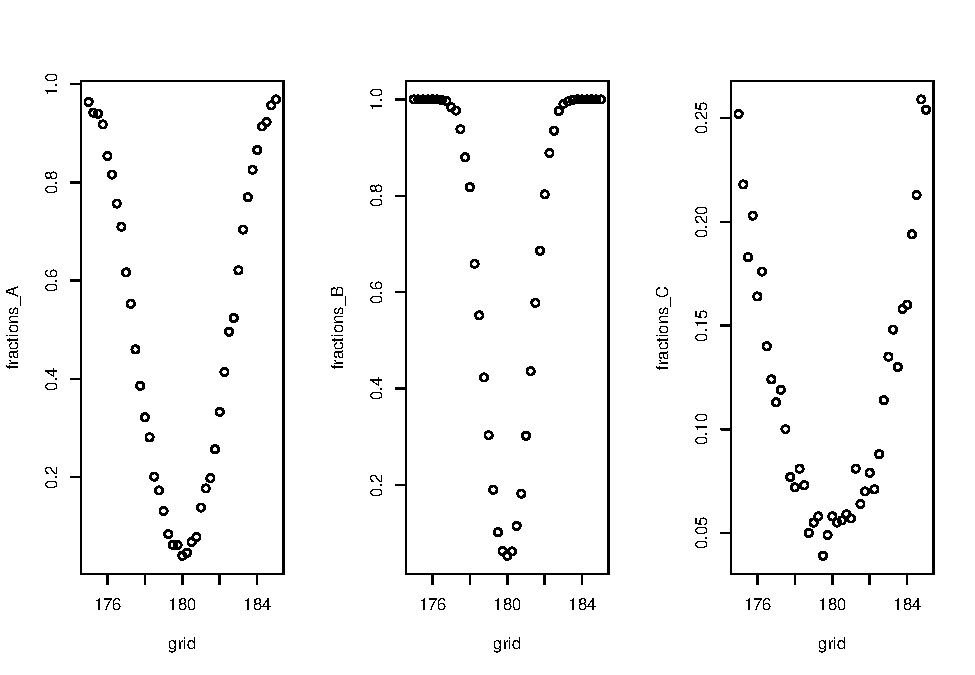
\includegraphics{Assignment-1_files/figure-latex/unnamed-chunk-6-1.pdf}

\hypertarget{d}{%
\subsection{d)}\label{d}}

The more datapoints seems to have an influence on the narrowness of the
plot. Furthermore, a bigger std gives a more wider distribution of
fractions as presented in the plot of C.

\hypertarget{exercise-3}{%
\section{Exercise 3}\label{exercise-3}}

\hypertarget{a-1}{%
\subsection{a)}\label{a-1}}

\begin{Shaded}
\begin{Highlighting}[]
\NormalTok{data}\OtherTok{\textless{}{-}}\FunctionTok{read.table}\NormalTok{(}\AttributeTok{file=}\StringTok{"data/telephone.txt"}\NormalTok{,}\AttributeTok{header=}\ConstantTok{TRUE}\NormalTok{)}
\NormalTok{data\_tele }\OtherTok{\textless{}{-}}\NormalTok{ data}\SpecialCharTok{$}\NormalTok{Bills}
\FunctionTok{par}\NormalTok{(}\AttributeTok{mfrow=}\FunctionTok{c}\NormalTok{(}\DecValTok{1}\NormalTok{,}\DecValTok{3}\NormalTok{))}
\FunctionTok{hist}\NormalTok{(data\_tele)}
\FunctionTok{qqnorm}\NormalTok{(data\_tele)}
\FunctionTok{boxplot}\NormalTok{(data\_tele)}
\end{Highlighting}
\end{Shaded}

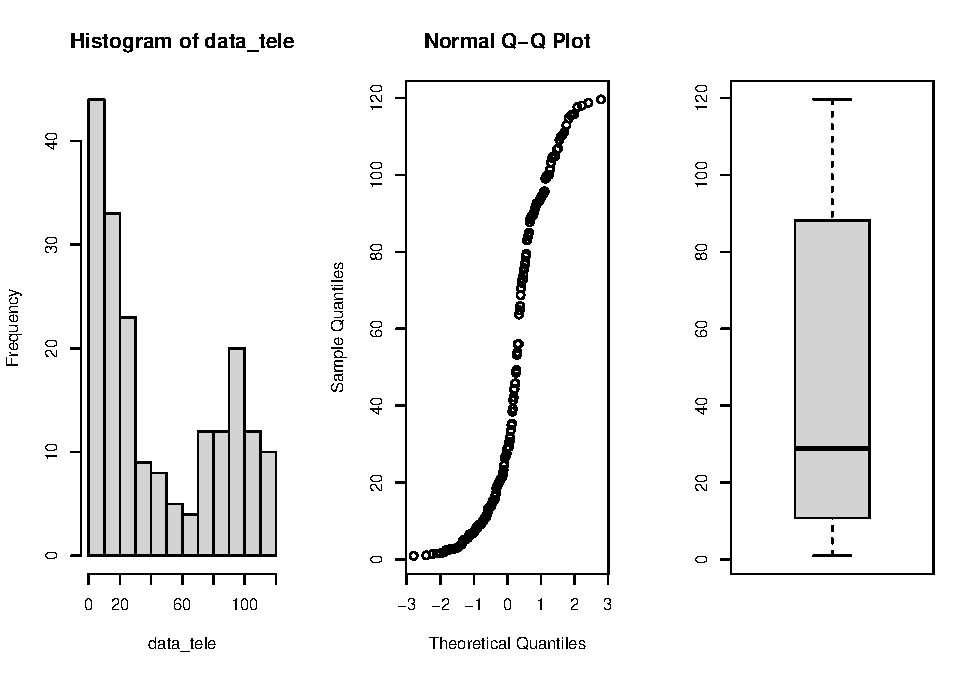
\includegraphics{Assignment-1_files/figure-latex/unnamed-chunk-7-1.pdf}

The data seems oddly distributed with two subpeaks, would have expected
a more normally distributed set. Therefore perhaps a good idea if the
manager arranges the prices better.

\hypertarget{b-1}{%
\subsection{b)}\label{b-1}}

\begin{Shaded}
\begin{Highlighting}[]
\NormalTok{X }\OtherTok{\textless{}{-}} \FunctionTok{seq}\NormalTok{(}\FloatTok{0.01}\NormalTok{, }\FloatTok{0.1}\NormalTok{, }\FloatTok{0.0005}\NormalTok{)}
\NormalTok{pvalues }\OtherTok{\textless{}{-}} \FunctionTok{c}\NormalTok{()}
\NormalTok{t }\OtherTok{\textless{}{-}} \FunctionTok{median}\NormalTok{(data\_tele)}
\ControlFlowTok{for}\NormalTok{ (x }\ControlFlowTok{in}\NormalTok{ X)\{}
\NormalTok{  B }\OtherTok{\textless{}{-}} \DecValTok{1000}
\NormalTok{  tstar }\OtherTok{\textless{}{-}} \FunctionTok{numeric}\NormalTok{(B)}
\NormalTok{  n }\OtherTok{\textless{}{-}} \FunctionTok{length}\NormalTok{(data\_tele)}
  
  \ControlFlowTok{for}\NormalTok{ (i }\ControlFlowTok{in} \DecValTok{1}\SpecialCharTok{:}\NormalTok{B)\{}
\NormalTok{    xstar }\OtherTok{\textless{}{-}} \FunctionTok{rexp}\NormalTok{(n,x)}
\NormalTok{    tstar[i] }\OtherTok{\textless{}{-}} \FunctionTok{median}\NormalTok{(xstar)}
\NormalTok{  \}}
\NormalTok{  pl}\OtherTok{\textless{}{-}}\FunctionTok{sum}\NormalTok{(tstar}\SpecialCharTok{\textless{}}\NormalTok{t)}\SpecialCharTok{/}\NormalTok{B}
\NormalTok{  pr}\OtherTok{\textless{}{-}}\FunctionTok{sum}\NormalTok{(tstar}\SpecialCharTok{\textgreater{}}\NormalTok{t)}\SpecialCharTok{/}\NormalTok{B}
\NormalTok{  p}\OtherTok{\textless{}{-}}\DecValTok{2}\SpecialCharTok{*}\FunctionTok{min}\NormalTok{(pl,pr)}
\NormalTok{  pl;pr;p}
\NormalTok{  pvalues }\OtherTok{\textless{}{-}} \FunctionTok{c}\NormalTok{(pvalues,p)}
\NormalTok{\}}
\CommentTok{\#pvalues}
\FunctionTok{plot}\NormalTok{(X, pvalues)}
\end{Highlighting}
\end{Shaded}

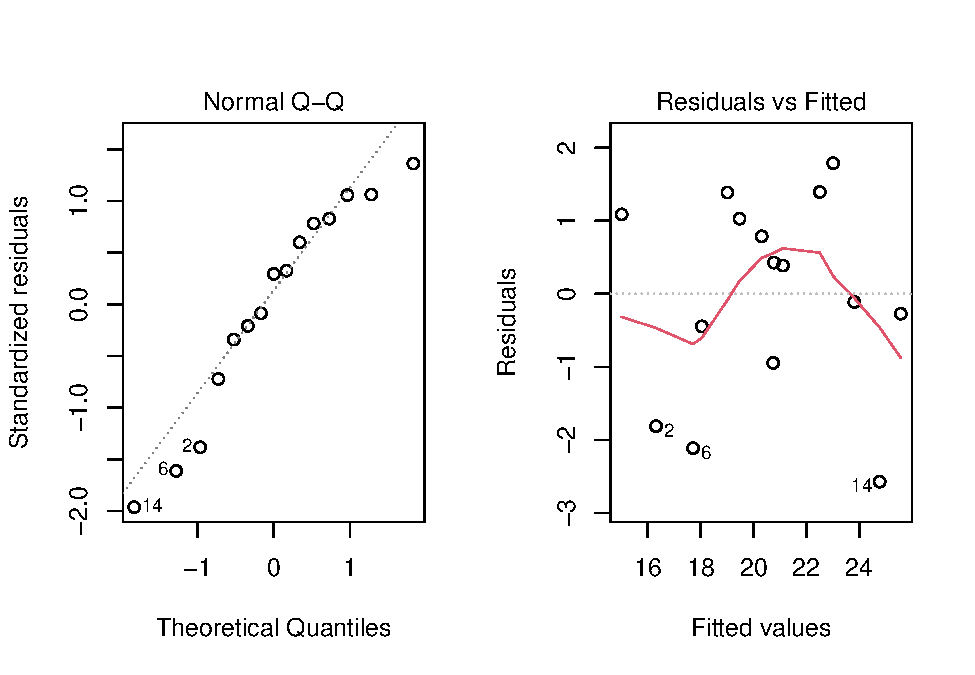
\includegraphics{Assignment-1_files/figure-latex/unnamed-chunk-8-1.pdf}
There exist an Exp function that fits the hypothesis

\hypertarget{c-1}{%
\subsection{c)}\label{c-1}}

\begin{Shaded}
\begin{Highlighting}[]
\NormalTok{B }\OtherTok{\textless{}{-}} \DecValTok{1000}
\NormalTok{T1 }\OtherTok{\textless{}{-}} \FunctionTok{median}\NormalTok{(data\_tele)}
\NormalTok{Tstar }\OtherTok{\textless{}{-}} \FunctionTok{numeric}\NormalTok{(B)}
\ControlFlowTok{for}\NormalTok{ (i }\ControlFlowTok{in} \DecValTok{1}\SpecialCharTok{:}\NormalTok{B)\{}
\NormalTok{  Xstar }\OtherTok{\textless{}{-}} \FunctionTok{sample}\NormalTok{(data\_tele,}\AttributeTok{replace=}\ConstantTok{TRUE}\NormalTok{)}
\NormalTok{  Tstar[i] }\OtherTok{\textless{}{-}} \FunctionTok{median}\NormalTok{(Xstar)}
\NormalTok{\}}
\NormalTok{Tstar25 }\OtherTok{\textless{}{-}} \FunctionTok{quantile}\NormalTok{(Tstar,}\FloatTok{0.025}\NormalTok{)}
\NormalTok{Tstar975 }\OtherTok{\textless{}{-}} \FunctionTok{quantile}\NormalTok{(Tstar, }\FloatTok{0.975}\NormalTok{)}

\NormalTok{T1}
\end{Highlighting}
\end{Shaded}

\begin{verbatim}
## [1] 26.905
\end{verbatim}

\begin{Shaded}
\begin{Highlighting}[]
\FunctionTok{c}\NormalTok{(}\DecValTok{2}\SpecialCharTok{*}\NormalTok{T1}\SpecialCharTok{{-}}\NormalTok{Tstar975, }\DecValTok{2}\SpecialCharTok{*}\NormalTok{T1}\SpecialCharTok{{-}}\NormalTok{Tstar25)}
\end{Highlighting}
\end{Shaded}

\begin{verbatim}
##    97.5%     2.5% 
## 19.29263 33.69000
\end{verbatim}

\hypertarget{d-1}{%
\subsection{d)}\label{d-1}}

\begin{Shaded}
\begin{Highlighting}[]
\NormalTok{max\_index }\OtherTok{\textless{}{-}} \FunctionTok{which.max}\NormalTok{(pvalues)}

\NormalTok{opt\_Lambda }\OtherTok{\textless{}{-}}\NormalTok{ X[max\_index]}
\end{Highlighting}
\end{Shaded}

The variable opt\_Lambda is the optimal lambda value with the highest
P-value.

\hypertarget{e}{%
\subsection{e)}\label{e}}

\begin{Shaded}
\begin{Highlighting}[]
\NormalTok{bill\_bigeq40 }\OtherTok{\textless{}{-}} \FunctionTok{sum}\NormalTok{(data\_tele}\SpecialCharTok{\textgreater{}=}\DecValTok{40}\NormalTok{)}
\NormalTok{bill\_smal40 }\OtherTok{\textless{}{-}} \FunctionTok{sum}\NormalTok{(data\_tele}\SpecialCharTok{\textless{}}\DecValTok{40}\NormalTok{)}

\FunctionTok{binom.test}\NormalTok{(bill\_bigeq40, }\FunctionTok{length}\NormalTok{(data\_tele),}\AttributeTok{p=}\FloatTok{0.5}\NormalTok{)}
\end{Highlighting}
\end{Shaded}

\begin{verbatim}
## 
##  Exact binomial test
## 
## data:  bill_bigeq40 and length(data_tele)
## number of successes = 83, number of trials = 200, p-value = 0.0194
## alternative hypothesis: true probability of success is not equal to 0.5
## 95 percent confidence interval:
##  0.3459337 0.4866247
## sample estimates:
## probability of success 
##                  0.415
\end{verbatim}

\begin{Shaded}
\begin{Highlighting}[]
\FunctionTok{binom.test}\NormalTok{(bill\_smal40, }\FunctionTok{length}\NormalTok{(data\_tele),}\AttributeTok{p=}\FloatTok{0.5}\NormalTok{)}
\end{Highlighting}
\end{Shaded}

\begin{verbatim}
## 
##  Exact binomial test
## 
## data:  bill_smal40 and length(data_tele)
## number of successes = 117, number of trials = 200, p-value = 0.0194
## alternative hypothesis: true probability of success is not equal to 0.5
## 95 percent confidence interval:
##  0.5133753 0.6540663
## sample estimates:
## probability of success 
##                  0.585
\end{verbatim}

\begin{Shaded}
\begin{Highlighting}[]
\NormalTok{bill\_less10 }\OtherTok{\textless{}{-}} \FunctionTok{sum}\NormalTok{(data\_tele }\SpecialCharTok{\textless{}} \DecValTok{10}\NormalTok{)}
\NormalTok{bill\_less10}\SpecialCharTok{/}\FunctionTok{length}\NormalTok{(data\_tele)}
\end{Highlighting}
\end{Shaded}

\begin{verbatim}
## [1] 0.26
\end{verbatim}

\hypertarget{exercise-4}{%
\section{Exercise 4}\label{exercise-4}}

\hypertarget{a-2}{%
\subsection{a)}\label{a-2}}

Disregarding the type of drink, test whether the run times before drink
and after are correlated.

\begin{Shaded}
\begin{Highlighting}[]
\NormalTok{data }\OtherTok{\textless{}{-}} \FunctionTok{read.table}\NormalTok{(}\AttributeTok{file=}\StringTok{"data/run.txt"}\NormalTok{,}\AttributeTok{header=}\ConstantTok{TRUE}\NormalTok{)}
\FunctionTok{cor}\NormalTok{(data}\SpecialCharTok{$}\NormalTok{before, data}\SpecialCharTok{$}\NormalTok{after)}
\end{Highlighting}
\end{Shaded}

\begin{verbatim}
## [1] 0.638803
\end{verbatim}

Run times before and after the drink seem to be positively correlated.

\hypertarget{b-2}{%
\subsection{b)}\label{b-2}}

\begin{Shaded}
\begin{Highlighting}[]
\CommentTok{\# calculate differences}
\NormalTok{data }\OtherTok{\textless{}{-}}\NormalTok{ data }\SpecialCharTok{\%\textgreater{}\%} 
  \FunctionTok{mutate}\NormalTok{(}\AttributeTok{diff =}\NormalTok{ before }\SpecialCharTok{{-}}\NormalTok{ after)}

\CommentTok{\# filter for lemo}

\NormalTok{lemo }\OtherTok{\textless{}{-}}\NormalTok{ data }\SpecialCharTok{\%\textgreater{}\%} 
  \FunctionTok{filter}\NormalTok{(drink }\SpecialCharTok{==} \StringTok{"lemo"}\NormalTok{)}

\FunctionTok{t.test}\NormalTok{(lemo}\SpecialCharTok{$}\NormalTok{before, lemo}\SpecialCharTok{$}\NormalTok{after, }\AttributeTok{paired =} \ConstantTok{TRUE}\NormalTok{)}
\end{Highlighting}
\end{Shaded}

\begin{verbatim}
## 
##  Paired t-test
## 
## data:  lemo$before and lemo$after
## t = -0.80596, df = 11, p-value = 0.4373
## alternative hypothesis: true difference in means is not equal to 0
## 95 percent confidence interval:
##  -0.5409781  0.2509781
## sample estimates:
## mean of the differences 
##                  -0.145
\end{verbatim}

\begin{Shaded}
\begin{Highlighting}[]
\CommentTok{\# filter for energy}

\NormalTok{energy }\OtherTok{\textless{}{-}}\NormalTok{ data }\SpecialCharTok{\%\textgreater{}\%} 
  \FunctionTok{filter}\NormalTok{(drink }\SpecialCharTok{==} \StringTok{"energy"}\NormalTok{)}

\FunctionTok{t.test}\NormalTok{(energy}\SpecialCharTok{$}\NormalTok{before, energy}\SpecialCharTok{$}\NormalTok{after, }\AttributeTok{paired =} \ConstantTok{TRUE}\NormalTok{)}
\end{Highlighting}
\end{Shaded}

\begin{verbatim}
## 
##  Paired t-test
## 
## data:  energy$before and energy$after
## t = 1.6538, df = 11, p-value = 0.1264
## alternative hypothesis: true difference in means is not equal to 0
## 95 percent confidence interval:
##  -0.05101059  0.35934392
## sample estimates:
## mean of the differences 
##               0.1541667
\end{verbatim}

For both energy and soft-drink groups there does not seem to be a
significant difference in running times.

\hypertarget{c-2}{%
\subsection{c)}\label{c-2}}

For each pupil compute the time difference between the two running
tasks. Test whether these time differences are effected by the type of
drink.

\begin{Shaded}
\begin{Highlighting}[]
\CommentTok{\# perform t{-}test}

\FunctionTok{t.test}\NormalTok{(lemo}\SpecialCharTok{$}\NormalTok{diff, energy}\SpecialCharTok{$}\NormalTok{diff)}
\end{Highlighting}
\end{Shaded}

\begin{verbatim}
## 
##  Welch Two Sample t-test
## 
## data:  lemo$diff and energy$diff
## t = -1.4764, df = 16.509, p-value = 0.1586
## alternative hypothesis: true difference in means is not equal to 0
## 95 percent confidence interval:
##  -0.7276409  0.1293076
## sample estimates:
##  mean of x  mean of y 
## -0.1450000  0.1541667
\end{verbatim}

The p-value is \textgreater{} 0.05 therefore the means of the two
populations are not significantly different.

\hypertarget{d-2}{%
\subsection{d)}\label{d-2}}

Can you think of a plausible objection to the design of the experiment
in b) if the main aim was to test whether drinking the energy drink
speeds up the running? Is there a similar objection to the design of the
experiment in c)? Comment on all your fndings in this exercise.

\hypertarget{exercise-5}{%
\section{Exercise 5}\label{exercise-5}}

\hypertarget{a-3}{%
\subsection{a)}\label{a-3}}

Test whether the distributions of the chicken weights for meatmeal and
sunflower groups are different by performing three tests: the two
samples t-test (argue whether the data are paired or not), the
Mann-Whitney test and the Kolmogorov-Smirnov test. Comment on your
fndings.

\begin{Shaded}
\begin{Highlighting}[]
\CommentTok{\# filter for meatmeal}

\NormalTok{meatmeal }\OtherTok{\textless{}{-}}\NormalTok{ chickwts }\SpecialCharTok{\%\textgreater{}\%} 
  \FunctionTok{filter}\NormalTok{(feed }\SpecialCharTok{==} \StringTok{"meatmeal"}\NormalTok{) }\SpecialCharTok{\%\textgreater{}\%} 
  \FunctionTok{select}\NormalTok{(weight)}

\CommentTok{\# filter for sunflower}

\NormalTok{sunflower }\OtherTok{\textless{}{-}}\NormalTok{ chickwts }\SpecialCharTok{\%\textgreater{}\%} 
  \FunctionTok{filter}\NormalTok{(feed }\SpecialCharTok{==} \StringTok{"sunflower"}\NormalTok{) }\SpecialCharTok{\%\textgreater{}\%} 
  \FunctionTok{select}\NormalTok{(weight)}

\CommentTok{\# check for data normality}

\FunctionTok{qqnorm}\NormalTok{(meatmeal}\SpecialCharTok{$}\NormalTok{weight)}
\end{Highlighting}
\end{Shaded}

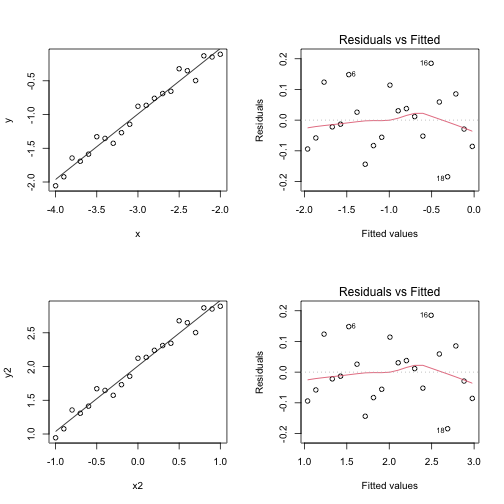
\includegraphics{Assignment-1_files/figure-latex/unnamed-chunk-15-1.pdf}

\begin{Shaded}
\begin{Highlighting}[]
\FunctionTok{qqnorm}\NormalTok{(sunflower}\SpecialCharTok{$}\NormalTok{weight)}
\end{Highlighting}
\end{Shaded}

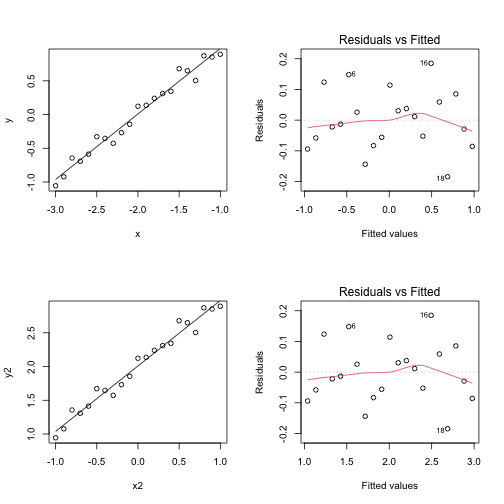
\includegraphics{Assignment-1_files/figure-latex/unnamed-chunk-15-2.pdf}

\begin{Shaded}
\begin{Highlighting}[]
\CommentTok{\# perform t{-}test, the data is not paired}

\FunctionTok{t.test}\NormalTok{(meatmeal, sunflower)}
\end{Highlighting}
\end{Shaded}

\begin{verbatim}
## 
##  Welch Two Sample t-test
## 
## data:  meatmeal and sunflower
## t = -2.1564, df = 18.535, p-value = 0.04441
## alternative hypothesis: true difference in means is not equal to 0
## 95 percent confidence interval:
##  -102.572435   -1.442716
## sample estimates:
## mean of x mean of y 
##  276.9091  328.9167
\end{verbatim}

\begin{Shaded}
\begin{Highlighting}[]
\CommentTok{\# Mann{-}Whitney test}

\FunctionTok{wilcox.test}\NormalTok{(meatmeal}\SpecialCharTok{$}\NormalTok{weight, sunflower}\SpecialCharTok{$}\NormalTok{weight)}
\end{Highlighting}
\end{Shaded}

\begin{verbatim}
## 
##  Wilcoxon rank sum exact test
## 
## data:  meatmeal$weight and sunflower$weight
## W = 36, p-value = 0.06882
## alternative hypothesis: true location shift is not equal to 0
\end{verbatim}

\begin{Shaded}
\begin{Highlighting}[]
\CommentTok{\# Kolmogorov{-}Smirnov test}

\FunctionTok{ks.test}\NormalTok{(meatmeal}\SpecialCharTok{$}\NormalTok{weight, sunflower}\SpecialCharTok{$}\NormalTok{weight)}
\end{Highlighting}
\end{Shaded}

\begin{verbatim}
## 
##  Two-sample Kolmogorov-Smirnov test
## 
## data:  meatmeal$weight and sunflower$weight
## D = 0.47727, p-value = 0.1085
## alternative hypothesis: two-sided
\end{verbatim}

Data in chickwts is not paired as the ``treatment'' of different feed
was applied to different newly-hatched chicks not the same chick. From
t-test we can see that the p-values \textless0.05, therefore the means
between the two groups are significantly different. From Mann-Whitney
test we can see that p-value is \textgreater0.05 therefore we can not
conclude that the medians of the two datasets are different. From
Kolgomorov-Smirnov test we can not conclude that the means are
different.

\hypertarget{b-3}{%
\subsection{b)}\label{b-3}}

Conduct a one-way ANOVA to determine whether the type of feed supplement
has an effect on the weight of the chicks. Give the estimated chick
weights for each of the six feed supplements. What is the best feed
supplement?

\begin{Shaded}
\begin{Highlighting}[]
\NormalTok{chickaov }\OtherTok{\textless{}{-}} \FunctionTok{lm}\NormalTok{(weight}\SpecialCharTok{\textasciitilde{}}\NormalTok{feed, }\AttributeTok{data =}\NormalTok{ chickwts)}
\CommentTok{\# performing one{-}way ANOVA}
\FunctionTok{anova}\NormalTok{(chickaov)}
\end{Highlighting}
\end{Shaded}

\begin{verbatim}
## Analysis of Variance Table
## 
## Response: weight
##           Df Sum Sq Mean Sq F value    Pr(>F)    
## feed       5 231129   46226  15.365 5.936e-10 ***
## Residuals 65 195556    3009                      
## ---
## Signif. codes:  0 '***' 0.001 '**' 0.01 '*' 0.05 '.' 0.1 ' ' 1
\end{verbatim}

\begin{Shaded}
\begin{Highlighting}[]
\CommentTok{\#extracting more information}
\NormalTok{summary\_table }\OtherTok{\textless{}{-}} \FunctionTok{summary}\NormalTok{(chickaov)}
\NormalTok{knitr}\SpecialCharTok{::}\FunctionTok{kable}\NormalTok{(}\FunctionTok{data.frame}\NormalTok{(summary\_table}\SpecialCharTok{$}\NormalTok{coefficients), }\StringTok{"latex"}\NormalTok{)}
\end{Highlighting}
\end{Shaded}

\begin{tabular}{l|r|r|r|r}
\hline
  & Estimate & Std..Error & t.value & Pr...t..\\
\hline
(Intercept) & 323.583333 & 15.83391 & 20.4360920 & 0.0000000\\
\hline
feedhorsebean & -163.383333 & 23.48549 & -6.9567776 & 0.0000000\\
\hline
feedlinseed & -104.833333 & 22.39254 & -4.6816194 & 0.0000149\\
\hline
feedmeatmeal & -46.674242 & 22.89580 & -2.0385502 & 0.0455667\\
\hline
feedsoybean & -77.154762 & 21.57799 & -3.5756235 & 0.0006654\\
\hline
feedsunflower & 5.333333 & 22.39254 & 0.2381746 & 0.8124949\\
\hline
\end{tabular}

From the results of one-way ANOVA we can see that the p-values is
\textless0.05 therefore we can conclude that the means between all of
the feed varieties are significantly different. From summary statistics
it seems that ``sunflower'' feed is the feed resulting in highest
weight. therefore it is the best.

\hypertarget{c-3}{%
\subsection{c)}\label{c-3}}

Check the ANOVA model assumptions by using relevant diagnostic tools.

\begin{Shaded}
\begin{Highlighting}[]
\CommentTok{\# check for normality}
\FunctionTok{qqnorm}\NormalTok{(chickaov}\SpecialCharTok{$}\NormalTok{residuals)}
\end{Highlighting}
\end{Shaded}

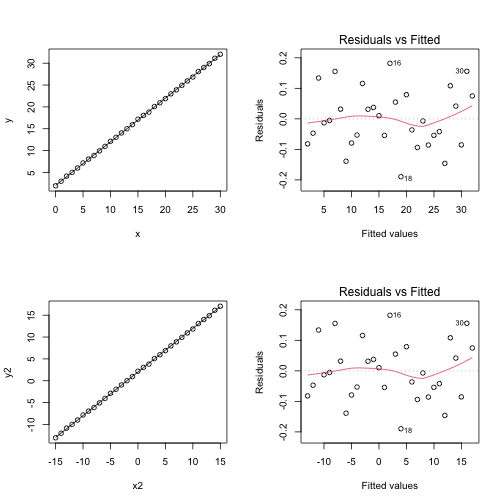
\includegraphics{Assignment-1_files/figure-latex/unnamed-chunk-17-1.pdf}

\begin{Shaded}
\begin{Highlighting}[]
\CommentTok{\# check if the variances are equal}
\NormalTok{chickwts }\SpecialCharTok{\%\textgreater{}\%} 
  \FunctionTok{group\_by}\NormalTok{(feed) }\SpecialCharTok{\%\textgreater{}\%} 
  \FunctionTok{summarise}\NormalTok{(}\AttributeTok{variance =} \FunctionTok{var}\NormalTok{(weight))}
\end{Highlighting}
\end{Shaded}

\begin{verbatim}
## # A tibble: 6 x 2
##   feed      variance
## * <fct>        <dbl>
## 1 casein       4152.
## 2 horsebean    1492.
## 3 linseed      2729.
## 4 meatmeal     4212.
## 5 soybean      2930.
## 6 sunflower    2385.
\end{verbatim}

From qqplot assumption of normality holds. However the assumption of
equal variances does not hold.

\hypertarget{d-3}{%
\subsection{d)}\label{d-3}}

Does the Kruskal-Wallis test arrive at the same conclusion about the
effect of feed supplement as the test in b)? Explain possible
differences between conclusions of the Kruskal-Wallis and ANOVA tests.

\begin{Shaded}
\begin{Highlighting}[]
\FunctionTok{kruskal.test}\NormalTok{(weight}\SpecialCharTok{\textasciitilde{}}\NormalTok{feed, }\AttributeTok{data =}\NormalTok{ chickwts)}
\end{Highlighting}
\end{Shaded}

\begin{verbatim}
## 
##  Kruskal-Wallis rank sum test
## 
## data:  weight by feed
## Kruskal-Wallis chi-squared = 37.343, df = 5, p-value = 5.113e-07
\end{verbatim}

With Kruskal-Wallis test we arrive to the same conclusion as with ANOVA.

\end{document}
